\documentclass[12pt,letterpaper]{article}
\usepackage[margin=0.75in]{geometry}
\usepackage{graphicx}
%\usepackage[bf,tiny,compact]{titlesec}
\usepackage{times}
\usepackage{xcolor}
\usepackage{xspace}
\usepackage{xstring}
%\usepackage{cite}
%\usepackage{natbib}
\usepackage[style=numeric,maxnames=5,minnames=3]{biblatex}
\usepackage{titlesec}
\usepackage{etoolbox}
\usepackage{wrapfig}
\usepackage{hyperref}


\makeatletter
\def\@maketitle{%
    {\centering\fontsize{12pt}{14pt}\selectfont\textbf{\@title}\par}
}
\patchcmd{\@footnotetext}{\footnotesize}{\fontsize{10pt}{12pt}\selectfont}{}{}
\makeatother

\addbibresource{refs.bib}

\renewcommand{\bibfont}{\fontsize{10pt}{12pt}\selectfont} % or any other  appropriate font command
\setlength\bibitemsep{0pt}
\defbibheading{bibliography}[\refname]{\noindent\textbf{#1}\vspace{-4pt}}
\DefineBibliographyStrings{english}{%
  references = {References (works to which I contributed have my name bolded)},
}

\titleformat{\section}{\normalfont\large\bfseries\scshape}{}{0em}{}
\titlespacing*{\section}{0em}{0.25\baselineskip}{0em}
\titleformat{\subsection}[runin]{\normalfont\normalsize\bfseries}{}{0em}{}[.]
\titlespacing*{\subsection}{0em}{0.25\baselineskip}{0.5em}


%% LOGIC FOR CUSTOMIZING THE STATEMENT FOR INDIVIDUAL SCHOOLS
% set up common defines (commands and boolean flags)
% Sets up custom commands and flags for school-specific behaviors
% Also assigns default values, but these can be overwritten with school-specific
% values in the corresponding header file.
% Some default values are placeholders (marked in red) and these MUST be 
% overwritten in the school-specific headers!
\newcommand{\schoolname}{\textcolor{red}{COLLEGE\_NAME}\xspace} 
\newcommand{\schoolnamelong}{\textcolor{red}{COLLEGE\_NAME\_LONG}\xspace}
\newcommand{\schooladdress}{\textcolor{red}{47 Generic St., City, ST 99999}\xspace}
\newcommand{\schoolintrocourses}{\textcolor{red}{[school-specific intro course numbers]}\xspace}
\newcommand{\schooladvcourses}{\textcolor{red}{[school-specific AI/ML/NLP course numbers]}\xspace}
\newcommand{\chairname}{\textcolor{red}{Prof. Search Chair}\xspace}
\newcommand{\chairlastname}{\textcolor{red}{Prof. Chair}\xspace}
\newcommand{\chairtitle}{\textcolor{red}{Chair, Faculty Search Committee}\xspace}
\newcommand{\department}{Department of Computer Science\xspace}
\newcommand{\position}{\textcolor{red}{POSITION\_NAME (POSITION\_ID)}\xspace}

\newif\iflongdei
\longdeitrue 
\newif\ifappendix
\appendixtrue 
\newif\ifliberalarts
\liberalartstrue

\newcommand{\materials}{my latest CV, a graduate transcript, and statements on teaching, research, and commitment to diversity and inclusion.\xspace}

\newcommand{\coverteachingpara}{%
\textcolor{red}{[school-specific segment on teaching philosophy]}
}

\newcommand{\coverresearchpara}{%
\textcolor{red}{[school-specific segment on research]}
}

\newcommand{\lateachingintro}{%
Liberal Arts education played a formative role in my approach to teaching---my love of teaching was first sparked during my undergraduate studies at Harvey Mudd College.
That was where I got my first (small) taste of what it is like to be an instructor, through my participation in the CS department's ``grutoring'' program---similar to TA positions found at larger universities, but with more emphasis on direct interaction with students.
This early experience of engaging directly with individual students, and seeing the specific things they struggled with, strongly influenced how I think about teaching.
To this day, I approach teaching by starting from a student's perspective: for any given course, what is a student most likely to struggle with, and what's the most effective way to help them understand it?
While the specific answers to these questions will naturally vary with each course and each student cohort, there are nevertheless a few concrete strategies which, broadly speaking, I have found to be good \emph{starting points} for any course: \textbf{teaching with narratives}, \textbf{leveraging technology for interactivity}, and \textbf{building inclusive learning environments}.%
}

\newcommand{\genteachingintro}{%
\textcolor{red}{TODO WRITE ME}
}

\newcommand{\lanarrativeend}{%
This makes it particularly valuable for a Liberal Arts setting, which emphasizes drawing connections between all parts of a student's education.
In such a setting, one way I could imagine explicitly drawing out such connections in an intro-level course would be to build narratives based on content from other core courses.
For example, using real problems faced in Digital Humanities as motivating examples for lectures would help connect the lecture content to students' core humanities coursework.
This approach has the potential to hit ``two birds with one stone'', advancing the College's mission while simultaneously grounding the core CS concepts to make them more approachable.%
}

\newcommand{\gennarrativeend}{%
\textcolor{red}{TODO WRITE ME}
}

\newcommand{\lainteractionend}{I believe this solution is particularly well suited to the small-class environment of a liberal arts college.}

\newcommand{\geninteractionend}{%
\textcolor{red}{TODO WRITE ME}
}

% import the school-specific header to make the magic happen!
% Not an actual school; meant to provide placeholder values
% for school-specific variables for the purposes of compiling
% generic versions of the statements
\renewcommand{\schoolname}{\textcolor{red}{COLLEGE\_NAME}\xspace}
\renewcommand{\schoolintrocourses}{\textcolor{red}{[school-specific intro course numbers]}\xspace}
\renewcommand{\schooladvcourses}{\textcolor{red}{[school-specific AI/ML/NLP course numbers]}\xspace}
\longdeitrue
\appendixtrue
\liberalartstrue
% link paragraph commands to the appropriate concrete implementation
\ifliberalarts
\newcommand\introclosing\laresearchintro
\newcommand\ugradclosing\laresearchclosing
\else
\newcommand\introclosing\genresearchintro
\newcommand\ugradclosing\genresearchclosing
\fi
%% END CUSTOMIZATION LOGIC

\title{Towards Computational Methods for Supporting Healthier Online Interactions}

\begin{document}
\maketitle

{\centering Research Statement --- Jonathan P. Chang \par}

\vspace{0.5\baselineskip}

\begin{wrapfigure}{r}{0.5\textwidth}
\centering
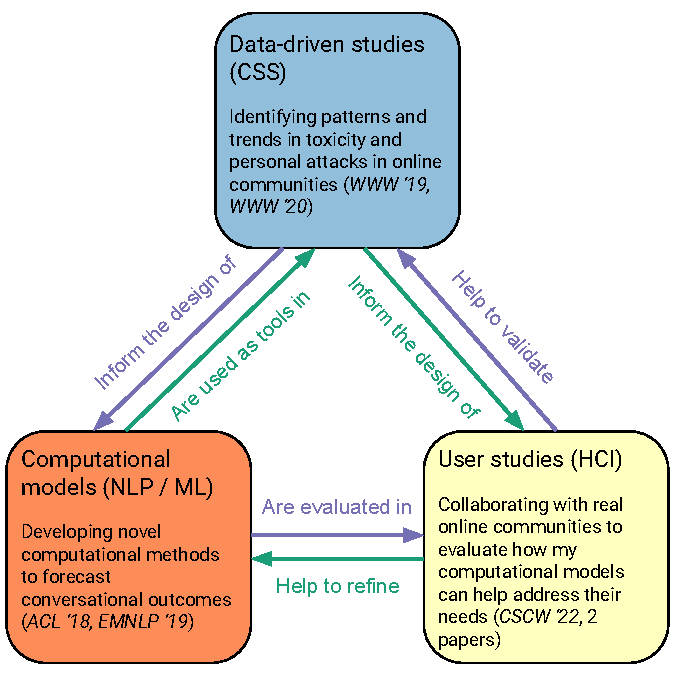
\includegraphics[width=0.48\textwidth]{FIG/the-circle-of-life.pdf}
\caption{My research agenda connects work across \textcolor{blue}{Computational Social Science (CSS)}, \textcolor{red}{Natural Language Processing (NLP) and Machine Learning (ML)}, and \textcolor{brown}{Human-Computer Interaction (HCI)}.}
\label{fig:research_overview}
\end{wrapfigure}

One of the biggest problems facing online platforms today is the prevalence of so-called ``toxic'' behavior, such as personal attacks, harassment, and general incivility.
While a lot of Computer Science research has responded to this problem by developing algorithms to detect toxicity, I argue that this approach implicitly centers the perspective of platform owners, who would be in a position to employ these algorithms for moderation, and leaves out an equally important perspective: that of the \emph{communities} of ordinary users who interact on these platforms.
Therefore, my research focuses on the following question: how can technology support members of online communities in having healthier interactions, and thereby prevent toxicity from taking root?
I tackle this question through a combined social and technical research agenda (Figure \ref{fig:research_overview}), in which I use both data-driven analysis and qualitative interviews to identify users' needs, pioneer new algorithmic methods to address those needs, and collaborate with real online communities to evaluate my new algorithmic methods in the wild and identify future research directions.
\introclosing

%\section{Background: The Landscape of Moderation}

%Popular discourse on content moderation tends to focus on the practices of social media companies, who often employ moderators to remove content deemed to be in violation of their (often opaque) rules.
%Yet a growing body of scholarship in social science and human-computer interaction argues that moderation actually encompasses a much richer body of practices extending all the way down to the community level \cite{brewer_inclusion_2020,seering_reconsidering_2020}.
%While moderation is commonly thought of as the purview of social media companies, who often employ moderators to remove content deemed to be in violation of their rules, social and political scientists have long recognized that many online communities also self-organize some less formal moderation practices \cite{grimmelmann_virtues_2015}.
%This community-driven moderation is often organized by volunteers, who play a role akin to a community leader \cite{seering_reconsidering_2020}.
%But these volunteer moderators do not act alone: they also involve ordinary community members in the moderation process, by engaging with the community to promote rule-following behavior through steps like publicly modeling good behavior, educating community members about the rules, and mediating discussions that are getting out of hand \cite{billings_understanding_2010,seering_shaping_2017}.
%These practices can be seen as \emph{proactive} moderation aimed at discouraging antisocial behavior from occurring at all---in contrast to \emph{reactive} moderation practices like content removal which respond to antisocial behavior after it occurs.

\section{My Research Contributions}
%My research aims to fill a gap in the existing Computer Science research on content moderation: while there has been a lot of work on computational tools to assist reactive moderation, such as algorithms to detect antisocial content and flag it for removal, I focus instead on the relatively understudied question of how computational methods can assist community-driven proactive moderation.

\subsection{Identifying Users' Needs}
Though toxicity is often thought of as the work of trolls, outside agitators, and other bad-faith actors, prior work has shown that even the ordinary, well-intentioned users that make up the majority of any online community can be influenced to engage in toxic behavior \cite{cheng_anyone_2017}.
As a first step in understanding how technology can help prevent this, I conducted data-driven studies to quantitatively examine the circumstances under which well-intentioned users are likely to turn toxic.
One study examining the Wikipedia editor community found evidence that users' attitudes towards a community's rules, such as whether they judge enforcement of the rules to be fair, can affect their willingness to follow them.
Another study, done as part of an internship at Facebook, showed that discussions in which a user was misperceived (i.e., the publicly perceived purpose of their message was different from what they intended) are more likely to turn toxic.
These results were published at the 2019 \cite{chang_trajectories_2019} and 2020 \cite{chang_dont_2020} meetings of The Web Conference (WWW '19 and '20), a top venue for social computing research.

To gain more qualitative insights about this phenomenon, I worked with undergraduate student Charlotte Schluger to interview Wikipedia administrators---the results of which were published at the 2022 ACM Conference on Computer-Supported Collaborative Work (CSCW '22) \cite{schluger_proactive_2022}, a top venue for research on online communities and human-computer interaction, with Charlotte as first author.
One key finding was that administrators reported that they can often intuitively tell when a currently-civil discussion is at risk of \emph{derailing} into toxicity---that is, they are able to pick up on early warning signs to \emph{forecast} derailment.
We subsequently posit that this represents a possible opening for computational assistance: if an algorithm could capture this same intuition to forecast derailment, it could be used to power just-in-time interventions warning users of the risk and encouraging them to keep the discussion on track.

\subsection{Demonstrating the Feasibility of Algorithmically Forecasting Derailment}
To test whether algorithmically forecasting derailment is feasible, I worked with industry partners
%at Alphabet and the Wikimedia Foundation 
to design an experiment studying algorithmic estimates of politeness, which has been theorized by socio-linguistics literature to be a mediating factor for avoiding conflict. We found that when polite language, as measured by machine learning models, was present early in a discussion, the discussion was at statistically significantly lower risk of derailment.
This work, presented at 2018 Annual Meeting of the Association for Computational Linguistics (ACL 2018; a leading venue for NLP research) \cite{zhang_conversations_2018}, established conversational forecasting as a new NLP task and established its feasibility, sparking follow-up work from other researchers attempting this task.\footnote{A partial list of papers attempting this task: \url{https://www.cs.cornell.edu/~jpchang/forecasting/}}

\subsection{Practical Forecasting of Conversational Derailment}
Classical machine learning approaches to natural language processing 
(like those in my earlier proof-of-concept work) 
typically operate on a fixed snapshot of a discussion, assuming it will never change.
But this is impractical for forecasting derailment in real moderation settings, because discussions evolve in real time: it is impossible to know in advance how many comments a discussion will get, and each new comment may increase or decrease the risk of derailment.
Thus, a practically useful algorithm would need to follow a conversation in real time, continuously updating its belief about whether the conversation is at risk of derailment.
In work presented at the ACL's 2019 Conference on Empirical Methods in Natural Language Processing (EMNLP 2019; a hub for debuting novel natural language models) \cite{chang_trouble_2019}, I developed such an algorithm, a neural network known as CRAFT, by adapting techniques from the domain of dialog modeling (aka ``chatbots''), where similar practical challenges are present.
Experiments on archived conversations from real online communities show that 77\% of discussions that actually derail are correctly detected by CRAFT (a standard machine learning evaluation metric known as recall); conversely, across all conversations where CRAFT predicts derailment, 64\% in fact go on to derail (a standard metric known as precision).

\subsection{Using Forecasting Algorithms to Support Users}
While CRAFT scores highly on standard machine learning metrics, these metrics do not necessarily translate into actual usefulness for humans.
To evaluate how forecasting algorithms like CRAFT can concretely benefit real online communities, I led a team of undergraduate and masters students to develop a prototype tool, ConvoWizard, that uses CRAFT to automatically warn users when a discussion they are replying to may be at risk of derailing into antisocial behavior.
ConvoWizard is now being tested in a series of user studies that were set up in collaboration with real online communities, ensuring that testing is done in a way that is respectful of community norms.

Though this work is still in progress, preliminary results published in CSCW 2022 \cite{chang_thread_2022} already offer promising signs of ConvoWizard's potential to improve online discussions.
Upon seeing warnings from ConvoWizard, users in the study tended to edit their comments in ways that decrease the (algorithmically-estimated) risk of derailment, unlike in a control condition where edits tended to increase the risk.
A linguistic analysis of the resulting comments showed that they exhibit increased use of known conflict avoidance strategies, such as adopting a more formal tone and asking questions.
Finally, in a feedback survey ConvoWizard users left largely positive evaluations of the tool: most notably, 54\% reported that ConvoWizard made them rethink posting a comment they might have later regretted, and 83\% expressed interest in long-term use of a ConvoWizard-style tool if it became publicly available.
%, and 64\% felt that if ConvoWizard were deployed at scale, the net effect would be an improvement in discussion quality.

\section{Future Directions}
I am a firm believer in the principle that before new technologies can be broadly adopted, we must first try to understand as fully as possible its ramifications for society and its potential risks.
%This is especially vital for work relating to content moderation, which is quickly becoming a major societal issue with implications for online safety, free speech, and social justice.
In line with this principle, the social aspect of my prior and ongoing work has been tailored towards understanding the impact of tools based on forecasting algorithms, so that any future large-scale deployment of such technology can be done in a responsible and ethical manner.
While the findings thus far have offered positive signs about the potential of this technology to improve online discussions, they also raise new questions about its limitations and possible improvements, which are the focus of my future plans.

\subsection{Improving the Transparency of Forecasting Algorithms}
The most common suggestion we received in the ConvoWizard exit survey was to improve the tool's \emph{transparency}.
Currently, when the tool reports that a discussion might be at risk of derailment, it does not explain why this might be the case.
Users reported that this sometimes made it difficult to decide how they should respond, especially when they disagreed with ConvoWizard's judgment.
Solving this problem will likely form the central focus of my research in the immediate future, and to this end I have already begun preliminary work to explore possible directions.
During Summer 2023, I worked with two undergraduate students to design new studies that will investigate how humans tend to judge the risk of derailment and what they would find helpful in an explanation of this risk.
I plan to use the insights from these studies, in combination with the latest technical innovations in explainable AI and text generation, to guide the development of next-generation conversational forecasting algorithms that can automatically generate human-readable explanations of their forecasts.

%But the transparency issue is not just a technical problem: it also ties in to the larger \emph{social} problem of algorithmic bias.
%By now, it has become well known that data-driven approaches are vulnerable to capturing biases embedded within the data.
%The question, then, is not whether forecasting algorithms like CRAFT contain biases---the answer is surely yes---but rather what kinds of biases exist and what their impact would be in a broadly deployed forecasting-based tool.
%This is uncharted territory, since most prior work on computational tools for moderation---and by extension, the analyses of their biases---focused on the reactive paradigm, and it is not clear how those findings might apply to proactive moderation.
%Like the rest of my research agenda, my plan for addressing this question is to take a combined social and technical approach.
%Once an explainable successor to CRAFT has been developed, my plan is to analyze the model's decisions through the lens of recent work from computational social science on codifying the social and power implications found in natural language \cite{sap_social_2020}.
%Cross-referencing this work with the model's decision-making processes could reveal, for instance, whether the algorithm is less sensitive to attacks towards specific underrepresented groups.
%And once such biases are identified, the same insights from social science could be applied to design ways to counter them.

\subsection{Incorporating Non-linguistic Context}
The models I have developed thus far look only at the linguistic content of the conversation itself to forecast whether the conversation will derail.
In practice, however, the trajectory of a conversation often depends on factors beyond what is directly said in the comments; for example, prior work has shown that a community member's willingness to adhere to community norms is influenced by how long they have been part of the community \cite{danescu-niculescu-mizil_no_2013}.
I am interested in investigating how recent breakthroughs in so-called multimodal models---that is, models capable of combining language data with other modes of input---could be adapted to enable forecasting algorithms to incorporate this non-linguistic context.
This is particularly important because toxicity is highly dependent on social context, and phenomena such as microaggressions and dogwhistles can alienate members of marginalized groups from a community despite not being overtly toxic.
Building on recent efforts to computationally model the social and power implications found in natural language \cite{sap_social_2020} could make forecasting algorithms more sensitive to social context, and thereby allow them to better serve marginalized groups.
%, reducing bias and improving equity in community-driven moderation.


\subsection{Measuring Longer-term Impacts}
Evaluations of ConvoWizard thus far have focused on the tool's immediate impact: that is, how seeing a warning when replying to an at-risk discussion impacts the user's behavior while writing the reply.
Looking forward, I also wish to understand what longer-term impacts such tools might have.
At a conversation level, we might ask whether a reply that was written with the help of ConvoWizard might lead to more pro-social behavior throughout the rest of the conversation, even among participants who don't have ConvoWizard.
At a community level, we must explore whether broad adoption of a tool like ConvoWizard improves the overall quality of discussions in the community (as 64\% of users in our exit survey felt it would), or instead leads to unintended negative side effects such as users becoming less willing to express any disagreement at all.
Answering these questions will require larger-scale, longer-term user studies, offering a chance for students to gain extended exposure to both computational social science research and the underlying software development challenges.

\section{Involving Undergraduates in my Research Agenda}
Throughout my research, I have had the pleasure and privilege of collaborating with several undergraduate students, who have contributed to my research agenda in a number of ways.
Most notably, two of my papers---the two CSCW papers---were co-authored with undergraduate student Charlotte Schluger, who is in fact first author on one of them.
She had the distinction of contributing through the entire research pipeline: she was part of the larger student team that implemented ConvoWizard, was responsible for both designing and conducting the interviews, and finally contributed large portions of the paper writing.
To me, Charlotte's experience illustrates the broad potential of my research agenda for undergraduates: it presents opportunities for both scientific contributions and software engineering contributions, offering valuable experience that is relevant to both academic and industry career paths.
%Moreover, I do not view these aspects as mutually exclusive: I believe that students interested in research can benefit from having to implement research ideas as usable software, and that students interested in going into industry can benefit from exposure to cutting-edge research ideas.

In fact, I have found through my past work with undergraduates that the software development components of my research agenda offer a solution to one of the biggest challenges in mentoring undergraduates: how to ease them into the world of research in an approachable way.
For many undergraduates starting research for the first time, research can seem intimidating because it is so different from what they have experienced before.
Unlike coursework and internship projects, which involve concrete tasks and clear deliverables, research is often very abstract and lacks clearly defined goals.
By having new students in my research group start with concrete software development tasks in projects like ConvoWizard, I give them a more familiar environment with clear deliverables through which progress can be tracked.
At the same time, as students work on these tasks, they gain exposure to the novel research ideas underlying the software, and hence these tasks serve as an accessible gateway to research.
This is well-illustrated by the experience of my first undergraduate mentee, Andrew Wang, who took an interest in social networks research that he was exposed to in his early work with me, and has since gone on to pursue research in this direction through the MS program at Stanford followed by the PhD program back here at Cornell.

My future research plans offer ample opportunities for me to carry out this mentoring strategy.
In addition to the ongoing ConvoWizard project, my plans for studying longer-term impacts of forecasting-based tools may involve the development of new tools catering to different needs and audiences.
Furthermore, I co-lead the development of ConvoKit \cite{chang_convokit_2020}, an open-source Python package for working with conversational data, which offers additional opportunities for starter projects.
I also believe such projects offer educational value even beyond research.
For one, they often involve concepts that undergraduates are exposed to in their CS coursework---such as class interface design, proper use of data structures, and reasoning about efficiency---and therefore provide a valuable supplement to their classroom learning.
And of course, students interested in industry careers can use these projects to gain valuable software engineering experience, as was the case for my mentee Caleb Chiam, who has become the largest contributor to ConvoKit.
\ugradclosing

\vspace{0.5\baselineskip}
\printbibliography

\end{document}
